\chapter{Objeto}
\section{Laboratório Ocean}

De forma a se aproximar de um dos principais nichos de seu interesse, a Samsung criou um programa de Relacionamento com Desenvolvedores, de forma a se aproximar de um grupo de profissionais que mais contribuem com a disseminação de novas tecnologias da Samsung. Esse programa possui diversas frentes, como o \textit{Developer Day}, que é um grande evento realizado uma vez por ano no Brasil e outros países da América Latina que visa promover as mais recentes tecnologias da marca, e o Laboratório Ocean, que visa a aproximação da comunidade estudantil e de startups em formação.

O Laboratório Ocean é uma iniciativa da Samsung que consiste em estimular desenvolvedores a criar soluções tecnológicas relacionadas aos produtos da marca coreana. A primeira sede do laboratório foi inaugurada em 2010 na Coréia do Sul, e a iniciativa foi replicada no Brasil há cerca de dois anos, com uma unidade em Manaus e outra em São Paulo. Ao passo que a unidade de Manaus foi estabelecida dentro da Universidade Estadual do Amazonas (UEA), a unidade de São Paulo encontrava-se até o fim de 2015 na Avenida Brigadeiro Faria Lima, uma das principais avenidas comerciais da cidade. Uma iniciativa recente movida por um ex-aluno, professores do departamento e o programa 'Parceiros da Poli' trouxe através de conversas informais a ideia de trazer o laboratório para dentro da USP. Como o modelo intra universitário funcionou bem em Manaus, foi decidido replicar o modelo e sediar o laboratório dentro da Universidade, hospedado dentro do Departamento de Engenharia de Produção (PRO).

O Ocean fornece dois tipos de cursos, básicos e intensivos. Os cursos básicos são de curta duração (aproximadamente 3 horas), e os cursos intensivos em seu módulo atual duram 4 meses, utilizando o espaço toda noite de segunda à quinta-feira. O foco inicial dos cursos foi o desenvolvimento em dispositivos móveis, em especial apoiados no sistema operacional Android, inerente aos aparelhos da Samsung, como o Galaxy S7. Com o passar do tempo, os cursos começaram a seguir as tendências de \textit{hardware} do mercado e consequentemente da própria Samsung, como \textit{wearables}, \textit{smart} TVs, Internet das Coisas e Realidade Virtual. Mesmo assim, a área de dispositivos móveis ainda representa 80\% dos cursos oferecidos por eles.

Os cursos curtos possuem como principal objetivo despertar o interesse de desenvolvedores em relação aos produtos da Samsung. Portanto, os cursos trabalham de forma a mostrar todos os produtos de alta tecnologia da samsung e capacitar desenvolvedores para que utilizem os seus dispositivos através do desenvolvimento de softwares. Para tal, é disseminado tanto o funcionamento dos \textit{Software Development Kits} (SDKs) da Samsung e suas APIs para permitir o acesso ao \textit{hardware} dos seus dispositivos quanto o uso do Android para manipulação do software na linguagem nativa atual do sistema operacional utilizado por eles. Para a execução desses cursos, a Samsung trabalha juntamente com empresas terceiras especialistas no assunto para preparar o material a ser passado. Algumas vezes funcionários da própria Samsung dão o treinamento, e em alguns momentos houve até participação do corpo docente da Poli.

Os cursos intensivos são cursos de pré-aceleração de empresas, e têm o intuito de fomentar o empreendedorismo, apesar de manter a base de disseminar o conhecimento em cima de produtos da Samsung. A empresa acredita que no atual mercado, a diferenciação competitiva sobre o \textit{hardware} está ficando cada vez mais difícil, por isso as empresas estão buscando se diferenciar frente às outras em conteúdo. Dentro desse contexto, a Samsung visa auxiliar empresas a se desenvolverem e elas - em contrapartida - auxiliam a enriquecer os produtos da Samsung, seja através de novos produtos ou através de serviços.

Dessa forma, os cursos de pré-aceleração procuram fornecer conhecimento e experiência ao desenvolvimento de suas empresas, através de mentorias, bate-papo, palestras e avaliações. Como são cursos gratuitos, um dos principais desafios é manter o próprio engajamento das empresas, por isso o motivo de haver encontros 4 vezes por semana, com mentoria, criação e gestão do projeto proposto pelo programa, com checkpoints de avaliação das empresas ao longo do projeto. Tudo isso feito de forma \textit{gamificada} dentro do próprio modelo. A primeira parte do programa consiste da validação do modelo de negócio proposto pela empresa, e a segunda parte corresponde à prototipação e desenvolvimento de produto de fato. Atualmente contribuem com esse programa os profissionais da Samsung, funcionários terceiros, professores da USP, membros do NEU e empresas parceiras (Sebrae, FIESP, IBM, Amazon).

A infraestrutura do laboratório consiste em uma grande sala para até 80 pessoas, porém caso necessário portas retráteis permitem a sua divisão em duas salas separadas. Essa estrutura fica aberta das 08 às 22 horas de segunda a sexta feira, podendo ser utilizada livremente pela comunidade estudantil da universidade, cedendo computadores e acesso a Wi-Fi de alta velocidade. As mesmas salas são utilizadas para a realização dos cursos mencionados anteriormente.

Por se tratar de um acordo entre a Samsung e o PRO, é necessário que sejam feitas reuniões de alinhamento das necessidades e expectativas entre partes, que não estão sendo realizadas nesse primeiro momento pois o projeto ainda está no início e não há conflitos aparentes. Entretanto a universidade também tem planos para o laboratório e acredita que o mesmo terá um grande impacto dentro e fora da universidade. Segundo as palavras do professor Eduardo Zancul na inauguração do Ocean: “É uma frente de ensino, pesquisa e extensão. Ensino pois será um espaço para disciplinas do curso de engenharia de produção; Pesquisa porque materiais e a estrutura do laboratório serão utilizados pela comunidade acadêmica; Extensão pois muitos cursos serão abertos para a comunidade”. O laboratório se tornou uma parceria de cogestão entre universidade e empresa que tem como principal mérito a geração de valor derivada da sinergia entre academia e indústria. 

\section{Identificação de Stakeholders do Laboratório}
\label{sec:identificacao_stakeholders}

De forma a ilustrar os principais stakeholders do laboratório representados nesse trabalho, foi criado um mapa representativos dos mesmos. 

\begin{figure}[h]
\caption{Mapa de stakeholders do projeto Ocean}
\centerline{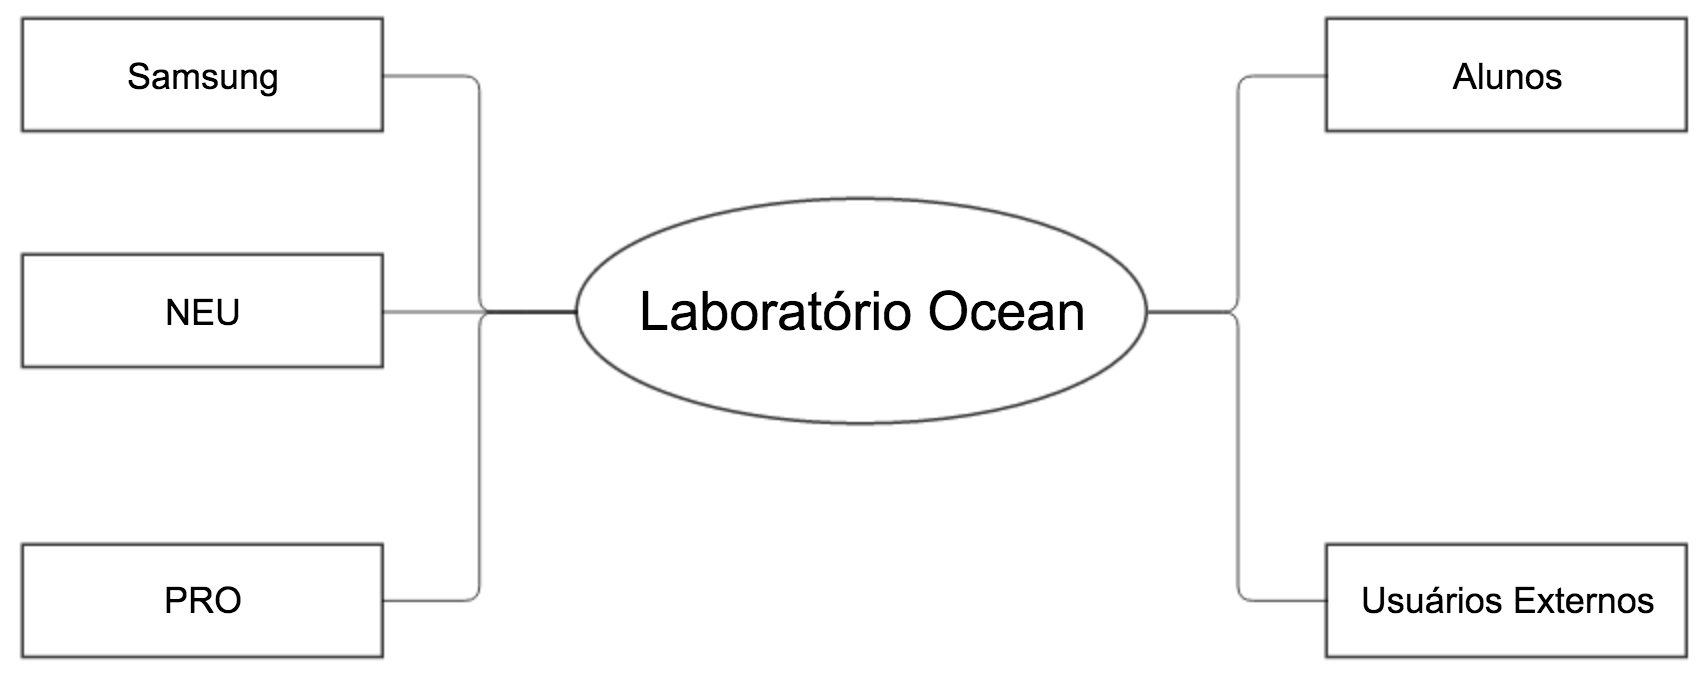
\includegraphics[scale=0.5]{img/stakeholders_v2}}
\label{fig:stakeholders}
\caption* {Fonte: Elaborado pelo próprio autor}
\end{figure}

\subsection{PRO}
\label{sec:con_pro}

O Ocean é um dos quatro grandes projetos que o PRO acompanha atualmente, esquematizado pela Tabela \ref{tab:pilares_pro}, juntamente com Inovalab, a Fábrica Didática e o Núcleo de Empreendedorismo da USP.

\begin{table}[H]
\begin{center}
\caption{Pilares do PRO}
\label{tab:pilares_pro}
{\def\arraystretch{2}\tabcolsep=10pt
\begin{tabular}{>{\raggedright}p{0.2\linewidth}>{\raggedright\arraybackslash}p{0.2\linewidth}>{\raggedright\arraybackslash}p{0.2\linewidth}>{\raggedright\arraybackslash}p{0.2\linewidth}}
\hline
     & Objetivo Institucional & Participação do PRO & Em Atividade  \\ \hline
     Inovalab & Laboratório de Inovação & Gestão Ativa & Sim  \\
     Fábrica Didática & Apropriação de conceitos de fábricas para aplicação no ensino & Em Desenvolvimento & Não \\
     Ocean & Laboratório de Desenvolvimento de Software & Cogestão com a Samsung & Sim \\
	 Núcleo de Empreendedorismo da USP & Disseminação da cultura empreendedora & Cede espaço físico & Sim \\ \hline
\end{tabular}%
}
\caption* {Fonte: Elaborado pelo autor em conversa com professores do departamento}
\end{center}
\end{table}

//Falar um pouco sobre cada um desses projetos, dar mais volume e explicar a importância do Ocean dentro desse contexto. 

\subsection{NEU}
\label{sec:con_neu}

O Núcleo de Empreendedorismo da USP é uma organização formada por alunos de graduação e pós-graduação, pesquisadores e professores que possuem a missão de promover a cultura de empreendedorismo dentro da Universidade. O NEU é aberto à toda comunidade da USP, já tendo recebido contribuições de diversas instituições da universidade, porém é formado atualmente principalmente por alunos da POLI e da FAU.

De forma similar ao estabelecimento do Ocean dentro do departamento do PRO, o NEU foi convidado a utilizar o espaço do Laboratório de Inovação (InovaLab) para sediar suas atividades. Atualmente o NEU trabalha com três principais pilares: inspiração, capacitação e conexão.

Inspiração diz respeito ao fomento ao empreendedorismo nos alunos para que eles se sintam impulsionados a participar do ecossistema de \textit{startups} ou até abrir as suas próprias. Portanto são feitos diversos convites aos diretores de diversas \textit{startups}, muitos com origens da própria USP, como Lean Survey, 99 Táxis e Squid, e estes podem explicar um pouco da sua trajetória e das emoções vividas graças aos seus empreendimentos. 

Capacitação é a frente do NEU de auxiliar ideias de alunos a se desenvolverem em produtos, para que assim sejam criadas novas empresas. A partir da rede de empresas que o NEU tem em seu leque de contatos, ele consegue encontrar mentorias para as empresas e acelerar o seu desenvolvimento. O principal programa dessa frente é o \textit{Startup Lab}, em que o NEU fornece material de apoio e mentoria através dos seus contatos com empresas, investidores e aceleradoras.

Conexão é representado principalmente pelo \textit{Startup Ship}, que é o canal do NEU destinado a alunos que querem estagiar em \textit{startups}. Através de sua rede de conexões ela facilita com que \textit{startups} e os alunos certos cheguem uns aos outros. Outro programa é o Pesquisas USP, que auxilia os alunos a se conectarem com pesquisas, e em contrapartida auxiliar pesquisadores a se conectarem com alunos ou empresas que possam auxiliar nos seus estudos. Nesse programa o NEU também auxilia startups a entrarem em contato com aceleradoras.

O NEU apresenta uma sinergia muito grande com o Ocean, pois ambos possuem muito interesse nessa fase de pré-aceleração de empresas, conseguindo exercer etapas distintas e complementares nesse processo. Durante os cursos intensivos do Ocean, o NEU se responsabiliza por trazer contatos de diferentes empresas para inspirar e fazer mentorias, ao passo que a Samsung trabalha fortemente na parte de capacitação e acompanhamento da evolução das empresas ao longo do programa.

Existe uma série de organismos dentro da universidade que fomentam a cultura de empreendedorismo, e como todos são gratuitos, existe uma colaboração muito grande para que os maiores beneficiados sejam as \textit{startups}, independente de  qual instituição que esteja contribuindo mais para a evolução da empresa.

\subsection{Alunos}
\label{sec:con_alunos}

A presença de um laboratório como este também ajuda a fomentar a cultura de empreendedorismo dentro da universidade, pois deixa os alunos próximos ao desenvolvimento de software, uma das principais bases de criação de novas \textit{startups}, devido ao baixo custo de aprendizado e investimento e alto valor gerado no curto e médio prazo. Ainda, segundo \citeonline{entrepreneurship}, os estudantes de engenharia experienciam o empreendedorismo de 4 maneiras: 

\begin{enumerate}
\item Primeiro passo para o auto-aprendizado
\item Preparação para a vida no trabalho
\item Caminho para ser autônomo
\item Desenvolvimento de liderança e responsabilidade de um time
\end{enumerate}

\subsection{Cursistas}
\label{sec:con_cursistas}

Conforme explicado anteriormente, o Ocean trabalha com duas propostas de cursos, os cursos básicos e os cursos intensivos. O primeiro modelo é de capacitação de desenvolvedores a trabalharem com dispositivos da Samsung, e o segundo modelo é para empreendedores que querem melhorar o modelo de negócio das suas propostas. Embora exista uma gama de pessoas que seja usuária de ambos os cursos - novos empreendedores têm muito interesse por programacão - o público-alvo de cada é diferente.

O primeiro modelo é desenhado para programadores ou aspirantes à programação. Embora existam diversos temas de cursos, o objetivo da Samsung é sempre de capacitar os cursistas a explorarem todas as capacidades permitidas pelo \textit{hardware} da Samsung. Para isso, serão explorados o sistema operacional Android, os SDKs da Samsung, o sistema operacional Tizen, em suma tudo que possa contribuir para o objetivo final. Portanto, é um curso de bastante interesse para todo tipo de pessoa que possui o desejo de desenvolver conteúdo que possa ser rodado em dispositivos da Samsung.

Segundo a 27\textsuperscript{a} Pesquisa de Anual do uso de TI, realizada pela Fundação Getúlio Vargas (FGV), o número de smartphones em uso no Brasil gira atualmente em torno de 168 milhões de dispositivos. \cite{tifgv}. Não obstante, além do alto número de smartphones, o Brasil também se mostra presente no mercado de outros dispositivos inteligentes, com previsão de movimentação de US\$4,1 bilhões no Brasil com IOT, segundo a assessoria de imprensa da IDC Brasil. \cite{idc}. Além do uso aplicado diretamente nessa área de dispositivos portáteis, a programação desenvolvida nessas atividades pode ser extendida para outras áreas de desenvolvimento, tornando os jovens mais capacitados para qualquer área tecnológica. Segundo a ONG Code.org, financiada por fundadores das maiores empresas de tecnologia do mundo como Mark Zuckerberg e Bill Gates, o número de empregos para programadores cresce exponencialmente, ao passo que o ensino de programação nas escolas não acompanha o mesmo ritmo, o que gerará uma falta de profissionais de TI em um futuro próximo. Juntamente a essa informação, o departamento de estatísticas de trabalho dos Estados Unidos (\textit{Bureau of Labor Statistics}) estima que o número de empregos para programadores dentro dos EUA diminuirá em até 8\%, pois mais profissionais deverão ser recrutados fora do país, devido ao baixo custo e a flexibilidade de trabalho remoto permitida pela programação. \cite{bls}

É nesse cenário de alto crescimento do uso de novas tecnologias no Brasil que o mesmo se mostra como um grande mercado para produtos inerentes ao uso de dispositivos inteligentes, como aplicativos e games. Dentro desse contexto, jovens interessados pelo desenvolvimento desse mercado no país se interessam por propostas como a do Ocean para realizar diferentes cursos nessas áreas.

Já em relação ao curso intensivo, o mesmo foi feito para incentivar ideias a se tornarem empresas, então é muito voltado para o nicho empreendedor, sem desapegar da área de tecnologia, que é de onde vêm toda \textit{expertise} da Samsung. Segundo \citeonline{empreendedorismo}, grande parte desse nicho empreendedor virá de universitários com as três principais características:

\begin{itemize}
\item Propensão a assumir riscos
\item Proximidade a outros empreendedores no círculo próximo
\item Já possuem uma ideia desenvolvida para o empreendimento
\end{itemize}

Logo, devido à localização e divulgação dentro da universidade, a maior parte dos cursistas do módulo intensivo virão de pessoas que possuem alguma laço com a universidade, como alunos e ex-alunos.